This thesis project extends and develops the original Distributed Software Development project, which have been created during the first semester of the 2021 / 2022 academic year. The original project aim was to create a system which could offer photogrammetry services, so the rendering of a tridimensional model from a set of images of the subject, leveraging the container technology to encapsulate the rendering engine. In this section I describe the original architecture of that system and in the next ones I will explain how that architecture has been redesigned, adapted and extended in this thesis project. 

\subsection{System Design}
\label{sse:originalsystemdesign}
  The MapNCloud project was designed as a "three plus one" tiers application:
  \begin{itemize}
    \item a \textbf{presentation layer} or front end, which has been developed as a web site and offers a graphical interface to the system
    \item a \textbf{business layer} or back end, which embodies all the business logic of the application
    \item a \textbf{data layer}, the database which persists the data needed by the application
    \item a \textbf{computation layer}, which is a separated back end module that is tasked with the most computational heavy routines (as the photogrammetry pipelines)
  \end{itemize}
  Another module is present in the application, and it is the ticketing service. It is not considered a whole tier, in fact its only job is to manage the queues of tasks that the backend generates, and let the computational layer components access them in the right order with the right schedule.
  \begin{figure}[H]
    \centering
    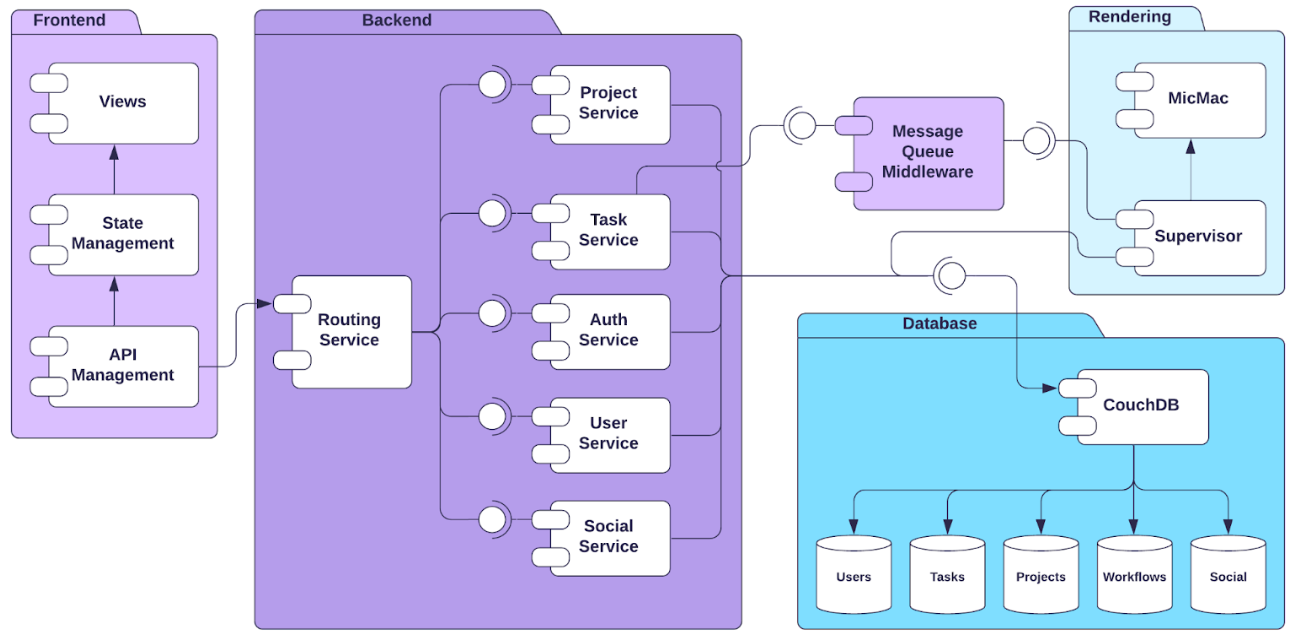
\includegraphics[width = \textwidth]{../Images/MNCOriginal.png}
    \caption{Original MapNCloud component diagram, with internal modules detailed.}
  \end{figure}

  \subsubsection{Front End}
  \label{ssse:originalfrontend}
    The presentation layer of the application was developed as a web application; this exposes a graphical user interface for the services offered by the system. It is a JavaScript application (developed with the VueJS framework) which interacts with the backend via HTTP calls; this allows it to be considered, by the cloud provider, a static web application, which is easy to deploy and has a low resources demand.\\
    The front end architecture follows the Model View ViewModel pattern, which separates the actual GUI elements from the logic of the user experience in View and ViewModel respectively, and lets the ViewModel reflect the changes on the Model; this is a common pattern to adopt as it provides a clear organization of functionalities and responsibilities among the internal software submodules.\\
    The front end is deployed as a static web app in the cloud provider web hosting dedicated service. It is directly built and made available from the code repository (through a CI/CD pipeline) reacting at every code change on a specific branch. The cloud provider also takes care of the SSL certificates (to ensure crypted communication) and the global availability through content delivery networks.\\
    The front end module is the one that is the least affected by this thesis work; it is only extended to include an administration section.

  \subsubsection{Back End}
  \label{ssse:originalbackend}
    The backend module is composed of two main software modules, which are distinct applications:
    \begin{itemize}
      \item the actual MapNCloud backend, a TypeScript application that exposes a REST API with all the functionalities of the application. This module is packaged as a Docker container; in this scenario, the possibility to bundle together code, configuration files and additional resources in a single Docker image makes deployment faster and easier, also providing all the isolation properties offered by the containers alone.
      \item a queue managing system, which acts as the ticketing system for the tasks issued to the computation layer. This is a RabbitMQ (a popular open source queue management system) instance, communicating via AMQP\cite{AMQP} with the other modules. The choice to separate these modules was taken to ensure the reliability of the whole system, and to enhance the maintainability of it (RabbitMQ offers out of the box monitoring services, which help to diagnose and follow the instance execution. These were to be reimplemented from scratch if the queuing module were implemented together with the application). This module is also deployed as a Docker container, but in this case the choice was made to reduce the amount of infrastructure needed for the application: the alternatives were deploying a single container group with RabbitMQ and the computational layer together or provisioning a whole virtual machine just for installing a whole instance of RabbitMQ.
    \end{itemize}
    The backend is the module that is most affected by this thesis work: in the next section the major changes will be analyzed, which affect the internal organization of components, the use of the tools offered by RabbitMQ and the positioning of the module in the overall architecture.
  
  \subsubsection{Data Layer}
  \label{ssse:originaldatalayer}
    The Data Layer is the component of the application that persists the data generated by the system, organizes it and make it available to the backend itself to distribute it. It is in charge of storing, as a example, the source files for the photogrammetry processes, the output 3D models, and all the data (stored as hierarchical text data) which describe the users, the projects and the tasks generated by the users themselves.\\
    The DB choice was CouchDB, a non relational database produced by Apache and is written in the same highly parallel technology of RabbitMQ; this also simplifies the deployment of clusters instead of single instances. The choice of non-relational was made to help in the earlier stage of development, where the flexibility of such an approach helped us in prototyping. As per the queuing system\ref{ssse:originalbackend}, this module is packaged, configured and deployed as Docker container.
    
  \subsubsection{Computation Later}
  \label{ssse:originalcomputationlayer}
    The "fourth layer" is the one that carries out the heavy computational tasks issued by the backend. It is composed by several independent \textit{workers}, which are simply containers, that are separated from the backend to ensure that it does not get stuck on a single request. These containers' internal architecture is rather simple: the chosen engine (during the original development MicMac) is wrapped in an external TypeScript application which divides the various phases of the pipeline in "Stages" and so extends the capability of the of the original engine: these Stages can be configured by the user (they are part of the data model memorized in the DB, in fact).\\
    The computational backend has to interact with the queuing system to retrieve the tasks and with the DB to get the resources and output the computed results. This "circular" dependency between backend modules is highlighted here because will be the cause of dome major change in the backend architecture. The container technology here is leveraged to ensure a fast spin-up time for a worker (which will be significantly longer for a VM, considering also the complex installation process of such engines) and the reusability of the images, which allows for a fast resize and scale of this layer of the architecture.
